% !TEX root = ../thesis_main.tex
\chapter{Properties of Single-Wall Carbon Nanotubes}

The properties of carbon nanotubes (CNT) strongly depend on their crystal structure. A CNT consists of carbon atoms bound together via sp$^2$ orbitals ($\sigma$ bonds) and arranged in a honeycomb lattice \cite{soavi2016ultrafast}. {\color{red} Distinguish DWCNTs, MWCNTs, and SWCNTs}. Due to the similarities between the crystal structures of graphene and CNTs, different CNT species can be classified using the basis vectors of the graphene lattice \cite{charlier2007electronic}. In fact, the countless ways of rolling up a graphene sheet into a nanotube evince that CNTs can exhibit varying helical geometries and symmetries with respect to their axial direction, as shown in Figure \ref{fig:symmetries}.

\begin{figure}[h]
	\centering
	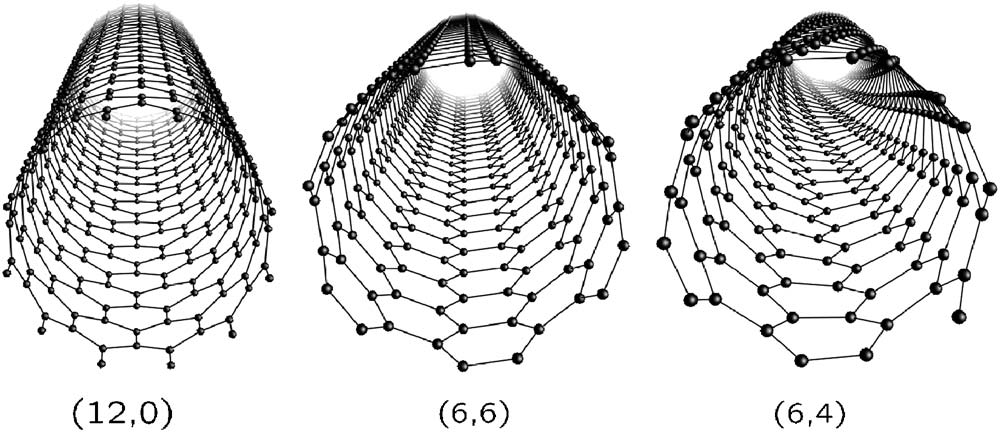
\includegraphics[scale=0.4]{images/chapter_optical_props/nanotube_symmetries_charlier}
	\caption{Crystal structures of (12,0), (6,6) and (6,4) single-wall carbon nanotubes. Reproduced from Ref. \cite{charlier2007electronic}.}
	\label{fig:symmetries}
\end{figure}
These morphological properties dictate the allowed electronic states by asserting boundary conditions on the electron wavefunction along the circumferential direction \cite{charlier2007electronic}. All allowed electronic states exhibit anisotropic features and obey a set of optical selection rules that govern allowed inter-band transitions. Moreover, the effect of strong electron-electron interactions impose further modifications to the electronic structure and effectively suppress the oscillator strengths associated with optical transitions involving any free-electron continuum states \cite{ando1997excitons}. This behavior distinguishes carbon nanotubes from conventional bulk semiconductors as they typically exhibit relatively weak Coulomb interactions \cite{ando1997excitons}.


\section{Definition of the Chiral Vector $\vec{C}_\text{h}$}

Each unique species of carbon nanotubes can be denoted using a set of indices ($m$,$n$). These integers $m$ and $n$ define the chiral vector $\vec{C_\text{h} }$ expressed as
\begin{equation}
	\vec{C_\text{h}} = n {\vec{a_\text{1}}} + m {\vec{a_2}} \equiv (m,n)
	\label{eq:chiral_vec}
\end{equation}
where $\vec{a_\text{1}}$ and $\vec{a_\text{2}}$ represent the lattice basis vectors of the 2D graphene sheet as shown in Figure \ref{fig:chiral_vectors}. This chiral vector $\vec{C_h}$ yields the nanotube diameter $d_t$ via the expression
\begin{equation}
	d_\text{t} = \dfrac{|\vec{C_\text{h}}|}{\pi} = \dfrac{a_\text{C-C}}{\pi}\sqrt{3(m^2 + mn + n^2)},
\end{equation}
where $a_\text{C-C} \approx$ \SI{1.44}{\angstrom} defines the nearest-neighbor distance between carbon atoms in graphene \cite{nanot2013single}.

\begin{figure}[ht]
	\centering
	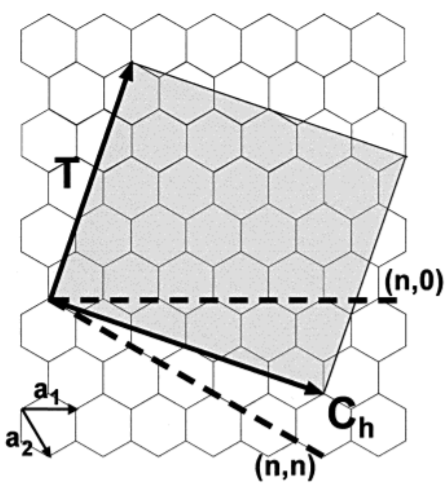
\includegraphics[scale=1]{images/chapter_optical_props/chiral_vectors_sheet.png}
	\caption{Two-dimensional graphene sheet featuring the lattice vectors $\vec{a_1}$ and $\vec{a_2}$ and the chiral vector $\vec{C_h}$ defined in Eq. \ref{eq:chiral_vec}. The vector $\vec{T}$ points in the axial direction of the carbon nanotube. Furthermore, $(n,n)$ and $(n,0)$ represent limiting cases for $\vec{C_h }$. Reproduced from Ref. \cite{odom2000structure}.}
	\label{fig:chiral_vectors}
\end{figure}


\section{Optical and Electronic Properties}

\subsection{Electronic Band Structure}

Given the similarities between CNTs and graphene, calculating the electronic band structure of graphene is the first step towards determining that of CNTs. A simple tight-binding model can be used to calculate the band structure of graphene. Such a model includes first nearest-neighbor interactions involving the $\pi$-orbitals of two atomic sites located at positions and $\vec{a}_1$ as well as $\vec{a}_2$ \cite{charlier2007electronic}. Here, $\vec{a}_1$ and $\vec{a}_2$ represent the lattice vectors of graphene. Furthermore, a hopping term $\gamma_0 \approx 2.9$ eV  characterizes the interactions between neighboring $\pi$-orbitals \cite{charlier2007electronic}. The Hamiltonian $\mathcal{H}$ for this simple system is then written as
%
\begin{equation}
	\mathcal{H} = \begin{bmatrix}
	0 & \alpha(k) \\
	\alpha^*(k) & 0
	\end{bmatrix}
\end{equation}
%
where $\alpha(\vec{k}) = (1 + e^{-i \vec{k}\cdot \vec{a_1}} + e^{-i \vec{k}\cdot \vec{a_2}})$ and $\alpha^*(\vec{k})$ refers to the complex conjugate of $\alpha(\vec{k})$\cite{charlier2007electronic}. In addition, $\vec{k}$ stands for a reciprocal space vector within the first Brillouin zone. Diagonalizing this matrix yields the energy dispersion
%
\begin{equation}
	E^{\pm} (k_\text{x}, k_\text{y}) = \pm \gamma_0 \sqrt{1 + 4 \cos\dfrac{\sqrt{3}k_\text{x} a}{2}\cos\dfrac{k_\text{y} a}{2} + 4 \cos^2 \dfrac{k_\text{y} a}{2}}
	\label{eq:graphene_band}
\end{equation}
 where $E^-$ and $E^+$ stand for the dispersion relations of the valence and conduction bands respectively. The variables $k_\text{x}$ and $k_\text{y}$ denote the x- and y-components of $\vec{k}$. Moreover, the constant $a = \sqrt{3}a_\text{C-C}$, where $a_\text{C-C} \approx$ \SI{1.44}{\angstrom} and refers to the nearest-neighbor distance between the lattice sites.
%
\begin{figure}[h]
	\centering
	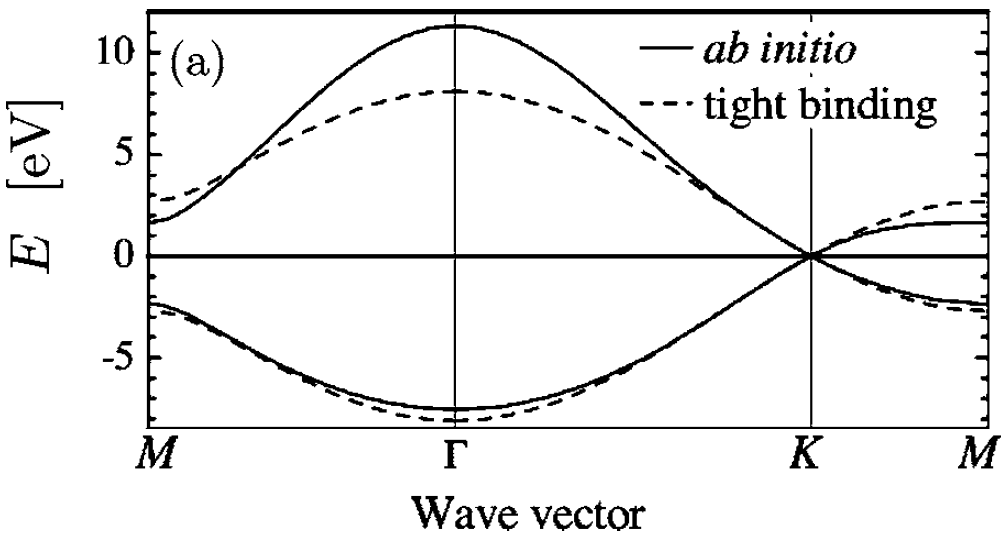
\includegraphics[scale=0.5]{images/chapter_optical_props/graphene_band_charlier}
	\caption{Electronic band structure of graphene determined using a tight-binding model (dashed line) and through ab-initio calculations (solid line). Reproduced and modified from Ref. \cite{reich2002tight}.}
	\label{fig:graphene_band}
\end{figure}
%
Figure \ref{fig:graphene_band} presents a plot of Eq. \ref{eq:graphene_band} as compared with a band structure calculation using ab-initio methods. Despite the disagreement between both approaches, they both predict a linear dispersion in the region near the $K$ position in momentum space \cite{charlier2007electronic}. This region of the band structure is commonly referred to as the Dirac cone	\cite{charlier2007electronic}. Moreover, both models identify graphene as a semimetal since the valence and conduction bands intersect at $K$ \cite{charlier2007electronic}. Without the presence of any dopants, the Fermi level remains exactly at the position where the two bands cross at K and the Fermi surface becomes an infinitesimal point. In conjunction with the band structure of graphene, the zone-folding approximation yields the band structure of CNTs.

\subsection{Chiralities of Semiconducting and Metallic Nanotubes}

The zone-folding method asserts that the periodic boundary conditions along the circumferential direction of CNTs dictate the quantization of the allowed $\vec{k}$ vectors in the electronic band structure \cite{charlier2007electronic}. This condition applied to the electron wavefunction $\Psi(\vec{r})$ is expressed as
\begin{equation}
\Psi_{\vec{k}}(\vec{r} + \vec{C_\text{h}}) = e^{i \vec{k} \cdot \vec{C_\text{h}}} \Psi_{\vec{k}}(\vec{r}) = \Psi_{\vec{k}}(\vec{r}),
\label{eq:boundary_cond}
\end{equation}
where $\vec{r}$ and $\vec{k}$ respectively define vectors in real and reciprocal space on the surface of the CNT \cite{charlier2007electronic}. Furthermore, $\vec{C_\text{h}}$ represents the chiral vector defined in Eq. \ref{eq:chiral_vec}. This condition gives the quantization of $\vec{k}$ which can be written as
\begin{equation}
	\vec{k} \cdot \vec{C}_h = 2\pi n
	\label{eq:quantization_cond}
\end{equation}
where n is an integer. Equation \ref{eq:quantization_cond} reveals that the symmetry of the CNT given by the chirality $\vec{C_\text{h}} \equiv (n,m)$ determines the band structure. Figure \ref{fig:k_quant} illustrates this. Depending on the chirality of the nanotube, the Dirac cone located at the K point may or may not be included the nanotube's bandstructure. This may determine whether or not the nanotube has a finite band gap energy.

\begin{figure}[h]
	\centering
	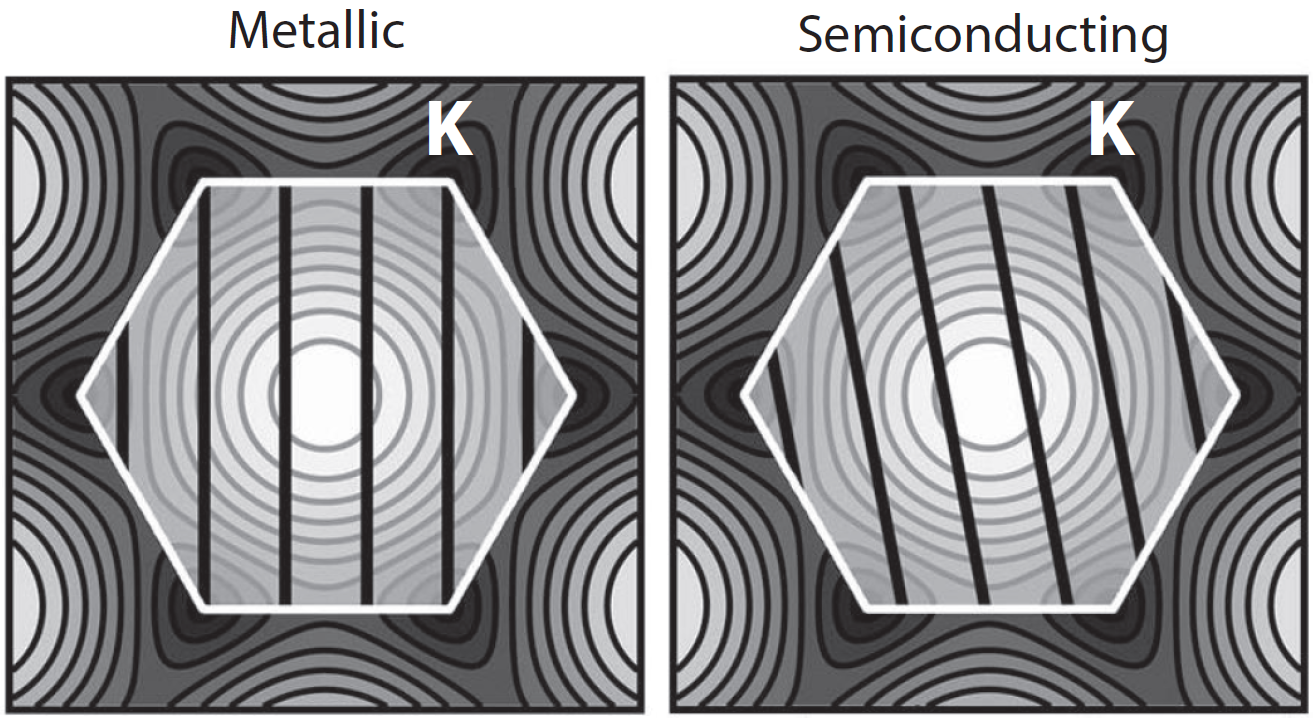
\includegraphics[scale=0.4]{images/chapter_optical_props/metal_semi_amori}
	\caption{The image shows the first Brillouin zone of graphene (white hexagon). The Dirac cone sites at the K point. Allowed values of $\vec{k}$ according to the quantization condition defined in Eq.\ \ref{eq:quantization_cond} are drawn over the Brillouin zone as thick, black, vertical lines. For metallic nanotubes, the electronic states located at the Dirac cone are allowed. Whereas, the band structures of semiconducting nanotubes do not include a Dirc cone. Reproduced from Ref.\ \cite{amori2018excitons}.}
	\label{fig:k_quant}
\end{figure}

In addition, the variable $\nu$ defined as
%
\begin{equation}
\label{eq:nu_cnt}
\nu \equiv (n-m) \mathrm{\hspace{1.5mm} mod \hspace{1.5mm}} 3,
\end{equation}
%
is also used to classify the two different band structures can occur.
%
\begin{figure}[h]
	\centering
	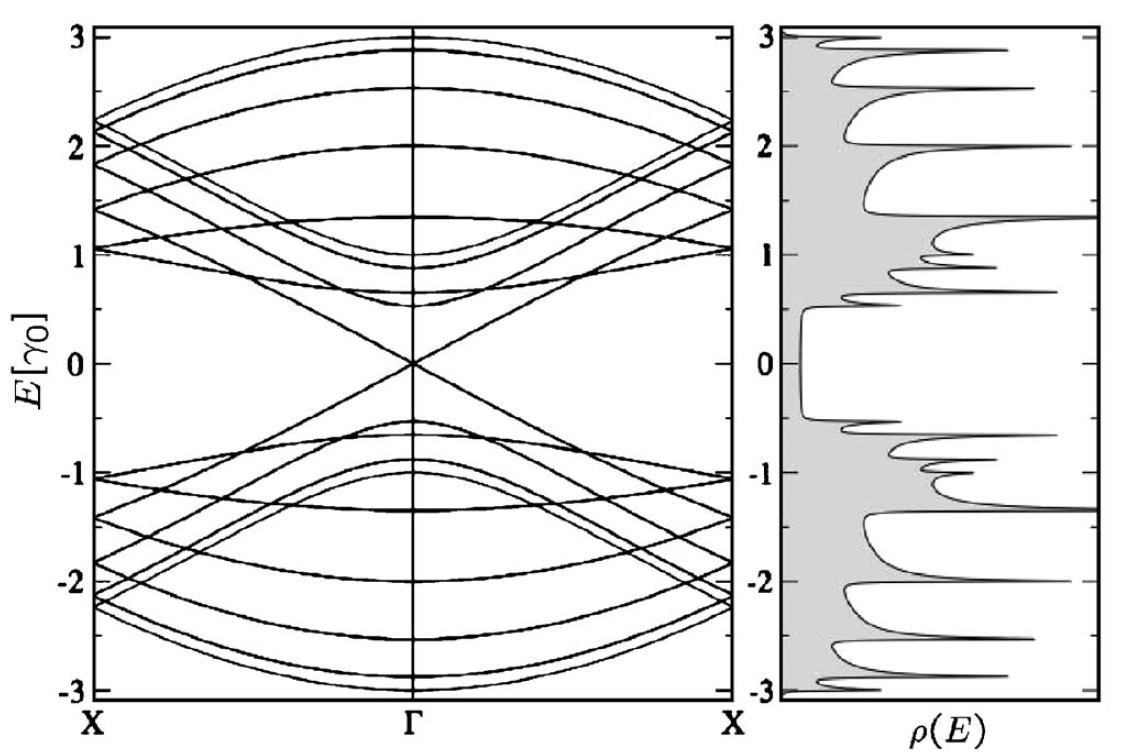
\includegraphics[scale=0.36]{images/chapter_optical_props/nine_zero_band_charlier}
	\caption{Band structure and density of states for a (9,0) carbon nanotube derived using the zone-folding scheme. These are plotted in units of $\gamma_0 \approx 2.9$, the tight-binding hopping energy between first nearest-neighbors. Reproduced from Ref.\ \cite{charlier2007electronic}.}
	\label{fig:nine_zero_cnt}
\end{figure}
%
In the case where $\nu = 0 $, the band structure contains a Dirac cone along with additional sub-bands within the valence and conduction bands as presented in Figure \ref{fig:nine_zero_cnt} . CNTs that satisfy this condition include $(n,n)$ carbon nanotubes, also commonly referred to as ``armchair'' nanotubes, that constitute the set of all metallic (gapless) nanotubes \cite{nanot2012optoelectronic}. Furthermore, $(n,m)$ nanotubes where $n-m = 3j$ ($j > 0$) also satisfy this $\nu = 0$ condition. However, these non-armchair nanotubes ($n\neq m$) exhibit curvature-induced band gaps and behave as narrow-gap semiconductors ($\sim1 - 100$ meV band gap energy) \cite{nanot2012optoelectronic}. {\color{red} What are curvature-induced band gaps?}

When $\nu= \pm 1$, the band structure corresponds to that of a medium-gap semiconductor ($\sim0.5 - 1$ eV band gap energy) \cite{nanot2012optoelectronic}. This band structure excludes the presence of a Dirac cone as shown in Figure \ref{fig:ten_zero_cnt}  \cite{charlier2007electronic}.

%\begin{figure}[h]
%	\centering
%	\begin{subfigure}{0.45\textwidth}
%		\centering
%		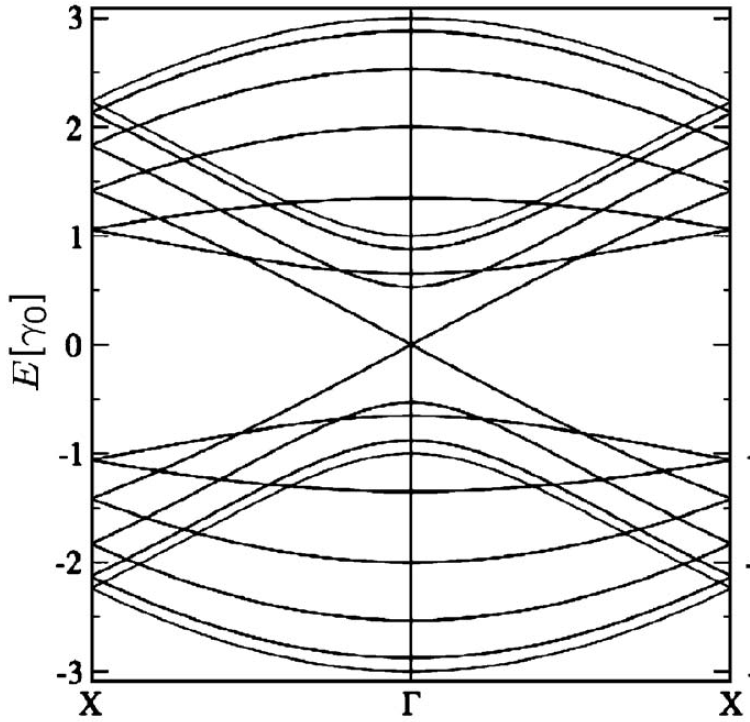
\includegraphics[scale=0.36]{images/chapter_optical_props/nine_zero_band_charlier_2}
%		\caption{Metallic}
%	\end{subfigure}
%	\qquad
%	\begin{subfigure}{0.45\textwidth}
%		\centering
%		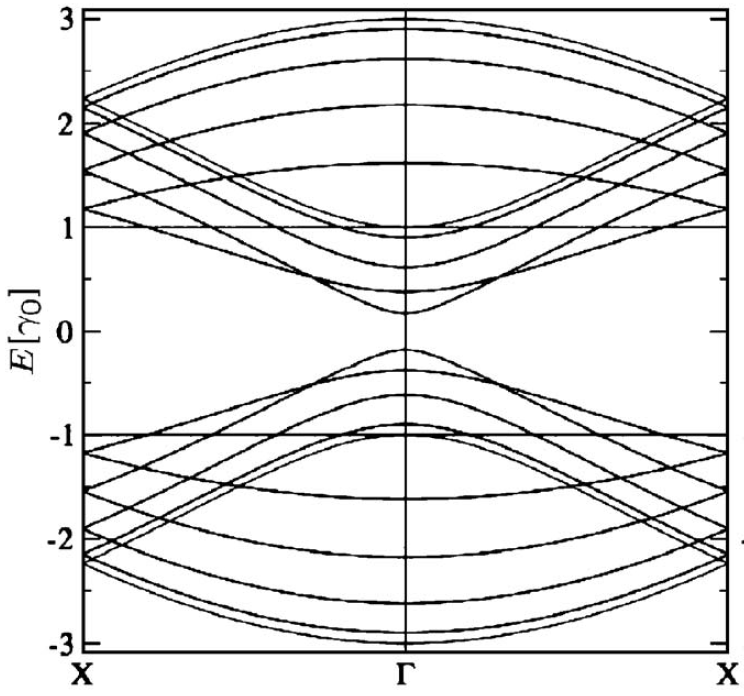
\includegraphics[scale=0.38]{images/chapter_optical_props/ten_zero_band_charlier_2}
%		\caption{Metallic}
%	\end{subfigure}
%	\caption{Reproduced and modified from Ref \cite{charlier2007electronic}.}
%\end{figure}


\begin{figure}[h]
	\centering
	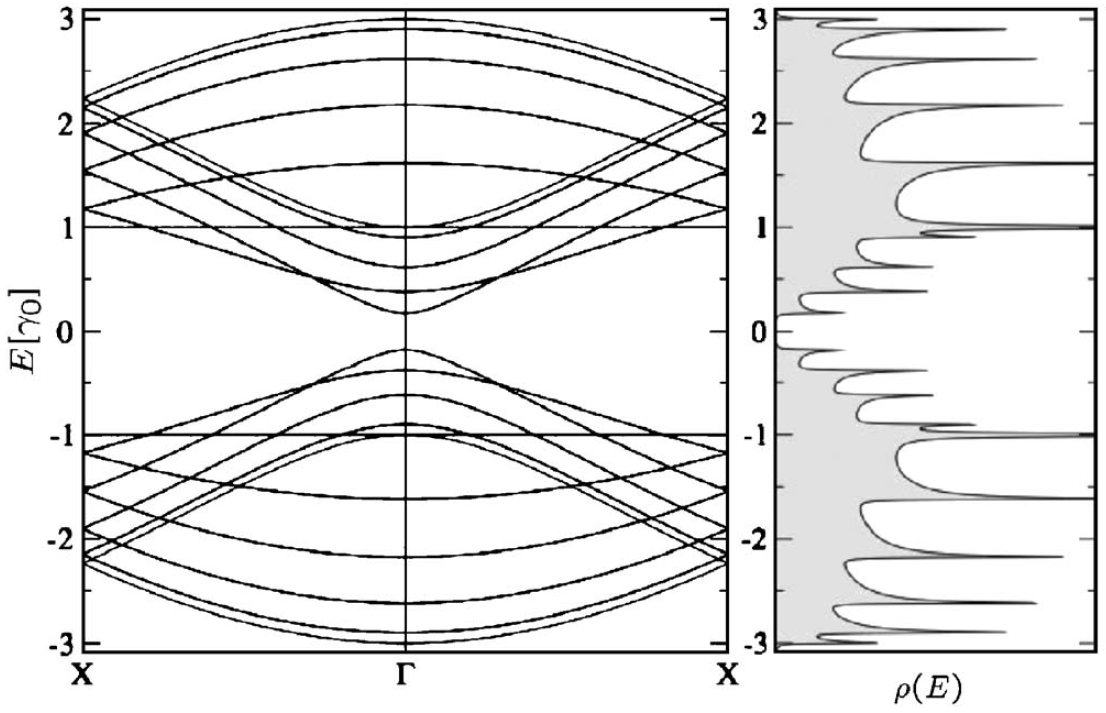
\includegraphics[scale=0.38]{images/chapter_optical_props/ten_zero_band_charlier}
	\caption{Band structure and density of states for a (10,0) carbon nanotube derived using the zone-folding scheme. These are plotted in units of $\gamma_0 \approx 2.9$ which represents the tight-binding hopping energy between first nearest-neighbors. Reproduced from \cite{charlier2007electronic}.}
	\label{fig:ten_zero_cnt}
\end{figure}


\subsection{Optical Selection Rules}
\label{section:selection_rules}
{\color{red} Explain where these come from}
Selection rules dictate the optical transitions that can occur. Such optical processes depend upon the conservation of both energy and angular momentum \cite{weismanKonoBook}. The notation E$_{ij}$ denotes an inter-band transition between the valence sub-band $i$ and the conduction sub-band $j$ \cite{weismanKonoBook}. In addition, $\Delta n \equiv i - j$ defines the difference between the band indices $i$ and $j$.  Incident light polarized parallel to carbon nanotube axial direction excites transitions where $\Delta n = 0$ \cite{weismanKonoBook}. This includes transitions such as $E_{11}$, $E_{22}$ and $E_{33}$. Whereas, incident light polarized perpendicular to the nanotube axial direction can only excite optical transitions where $\Delta n = \pm 1$ such as $E_{12}$ \cite{weismanKonoBook}.

\begin{figure}[h]
	\centering
	\begin{subfigure}{\textwidth}
		\centering
		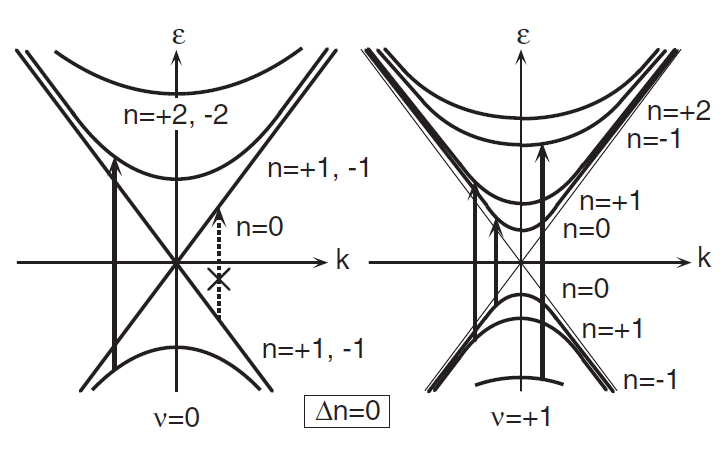
\includegraphics[scale=0.65]{images/chapter_optical_props/selection_rules_1.png}
		\caption{Selection Rules for light polarized parallel to the axial direction of carbon nanotubes. In the $\nu=0$ case, transitions within the Dirac cone are forbidden.}
	\end{subfigure}
	\begin{subfigure}{\textwidth}
		\centering
		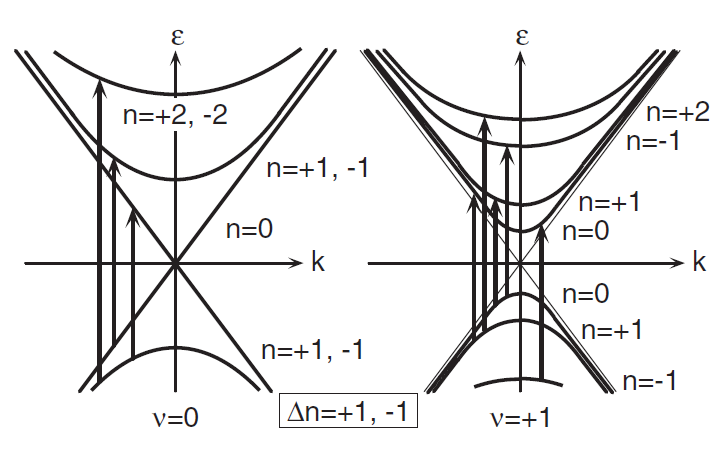
\includegraphics[scale=0.65]{images/chapter_optical_props/selection_rules_2.png}
		\caption{Selection Rules for light polarized perpendicular to the axial direction of carbon nanotubes.}
	\end{subfigure}
	\caption{Optical selection rules for metallic and narrow-gap semiconducting nanotubes ($\nu = 0 $) as well as medium-gap semiconducting nanotubes ($\nu = \pm 1$) . Reproduced from Ref.\ \cite{ando2005theory}.}
	\label{fig:selection_rules}
\end{figure}

\section{Excitons in SWCNTs}

\subsection{The Supression of Optical Transitions Involving the Free-Electron Continuum}
The simple tight-binding picture presented earlier ignores the effects of electron-electron interactions and thereby does not fully account for the effects of quantum confinement \cite{weismanKonoBook}. Indeed, the inclusion of electron-electron interactions into this picture yields a new electronic structure in which free electrons play a minimal role.

Strong electron-electron interactions influence the binding energies of quasi-particles known as excitons that form after the creation of an electron-hole pair \cite{koch2006semiconductor}. Excitons represent hydrogen-like quasi-particles composed of a negatively-charged electron bound to a positively-charged hole \cite{koch2006semiconductor}. In an ideal 1-D material, theory predicts that excitons will have an infinite binding energy \cite{ando2005theory}. This alone foreshadows the dominance of excitons in the optical properties of carbon nanotubes \cite{ando2005theory}.

\begin{figure}[h]
	\centering
	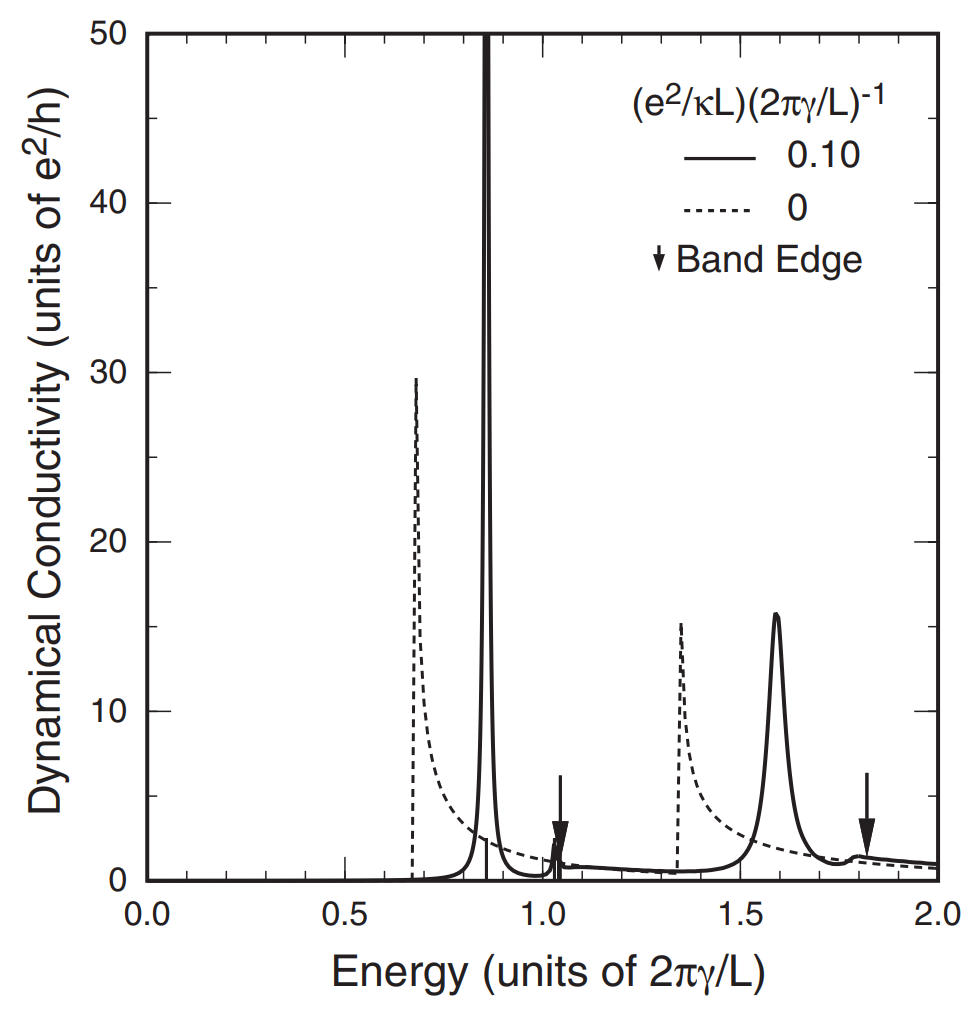
\includegraphics[scale=0.35]{images/chapter_optical_props/ando_suppression}
	\caption{Optical absorption spectrum of a semiconducting nanotube with (solid line) and without (dashed line) the effect of Coulomb interactions. Arrows mark the band edge positions of free electron continua. Reproduced and modified from Ref.\ \cite{ando2005theory}.}
	\label{fig:ando_suppression}
\end{figure}

The strong quantum confinement of nanotubes effectively suppresses the density of states of any free electron continuum whilst enhancing that of excitonic states. Moreover, the effective strength of Coulomb interactions $S_\text{e-e}$ can be expressed as
\begin{equation}
	S_\text{e-e} \equiv \dfrac{e^2 \kappa / L}{2 \pi \gamma / L},
\end{equation}

where $e^2 /\kappa L$ and $2 \pi \gamma / L$ account for the characteristic energy scales associated with Coulomb interactions and the kinetic energy of electrons respectively \cite{ando2005theory}. Here, $e$ defines the charge of an electron, $\gamma$ represents a band parameter, $L$ indicates the nanotube circumference $|\vec{C}_\text{h}|$, and $\kappa$ denotes the static dielectric constant used to account for screening effects.

Figure \ref{fig:ando_suppression} shows the calculated optical absorption spectrum of a semiconducting nanotube with and without the presence of Coulomb interactions. The plot shows the presence of van Hove singularities when ignoring the effect of Coulomb interactions. After accounting for these interactions, the oscillator strength of the low energy bound states of excitons becomes enhanced and absorption in the free-electron continuum drastically diminishes. The band edge of the free-electron continuum also shifts as a result of Coulomb interactions \cite{ando1997excitons}. Furthermore, this shift of the band edge increases as $S_{e-e}$ increases \cite{ando2005theory}.

\begin{figure}[h]
	\centering
	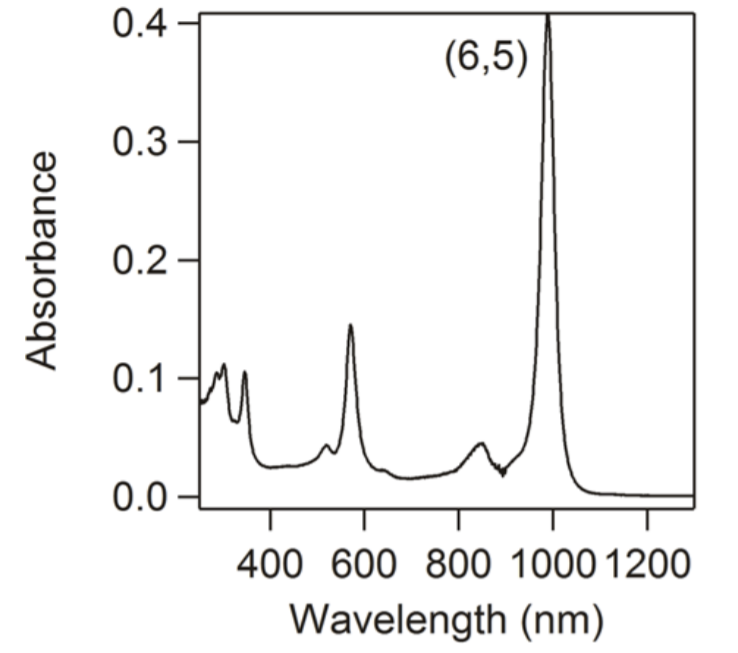
\includegraphics[scale=0.62]{images/chapter_optical_props/cnt_absorbance_yota}
	\caption{Absorbance spectrum of a (6,5) carbon nanotube sample at room temperature. The peaks at 983 and 570 nm correspond to the $E_{11}$ and $E_{22}$ of (6,5) carbon nanotubes. The $E_{12}$ transition of (6,5) nanotubes can also be observed at 650 nm. Reproduced from Ref.\ \cite{ichinose2017extraction}. }
	\label{fig:cnt_abs_yota}
\end{figure}

\subsection{Exciton Binding Energies}

In essence, the exciton binding energy characterizes the strength of the Coulomb interaction between an electron as well as its corresponding hole \cite{valkunas2006exciton}. On one hand, if the exciton binding energy is smaller than the thermal energy $k_b T$, then this Coulomb interaction becomes negligible \cite{valkunas2006exciton}. This causes electrons and holes to behave independently of each other. On the other hand, if the binding energy is much higher than the thermal energy, then electrons and holes tend to form stable, charge-neutral excitons \cite{valkunas2006exciton}.

The binding energies of excitons in CNTs tend to be on the order of hundreds of meV \cite{wang2005optical}. For instance, the excitons of (6,5) nanotubes have a binding energy of roughly 400 meV \cite{wang2005optical}. At room temperature $k_b T \approx$ 26 meV, meaning that the energy scale associated with thermal fluctuations falls short of the exciton binding energies in CNTs. Thus, excitons of CNTs are quite stable at room temperature. Figure \ref{fig:cnt_abs_yota} illustrates this effect as the room-temperature absorbance spectrum of a (6,5) sample exhibits well-defined, excitonic resonances {\color{red} How can we tell that these are excitonic resonances? Cite Feng Wang Paper}.

In contrast, conventional semiconductors such as GaAs only exhibit excitons with binding energies typically less than 20 meV \cite{liang1970excitons}.  As a result, these materials have to be cooled down to low temperatures in order to easily observe exciton resonances as shown in Figure \ref{fig:gaas_vs_cnt_absorbance}.

\begin{figure}[h]
	\centering
	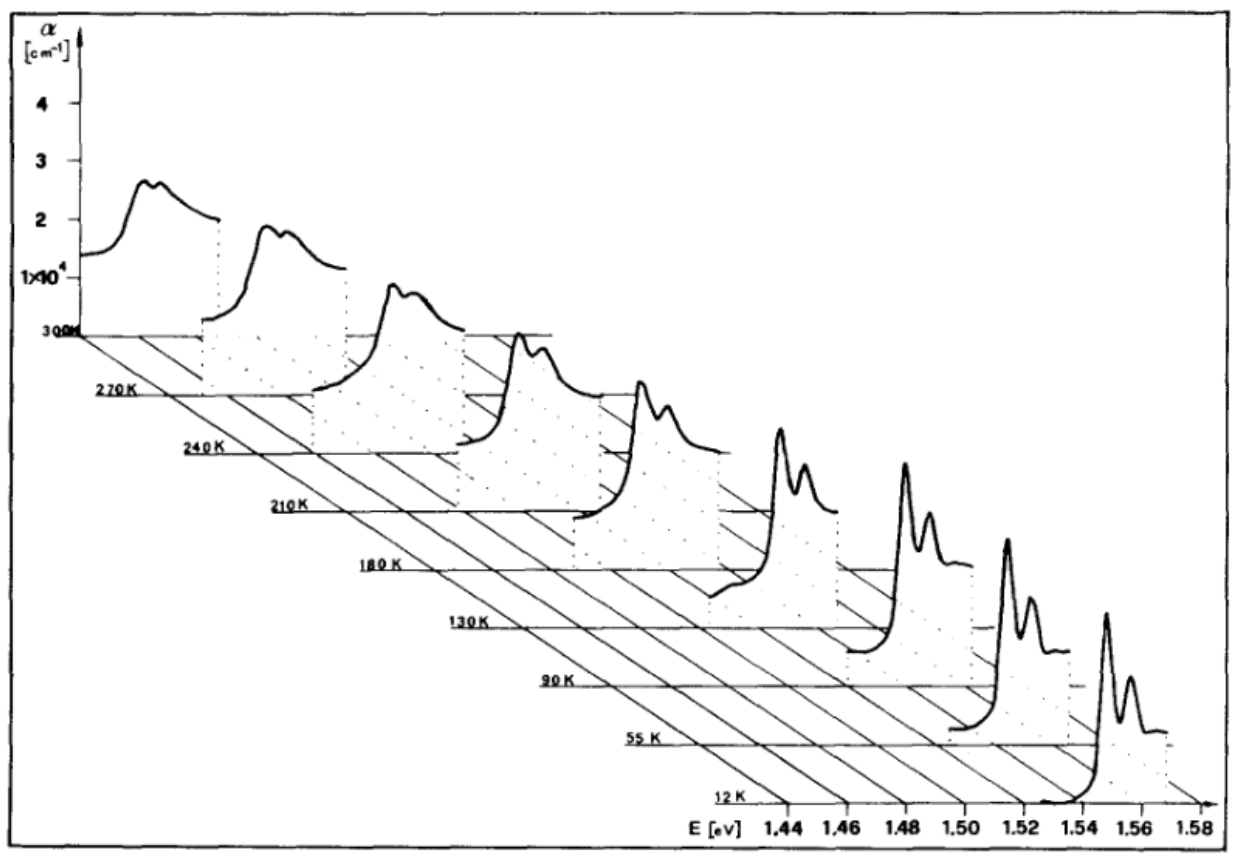
\includegraphics[scale=0.55]{images/chapter_optical_props/gaas_absorbance_filipowicz}
	\caption{GaAs/AlGaAs quantum well absorbance spectra at different temperatures. At higher temperatures, the presence of excitonic resonances is diminished. As the temperature decreases, two exciton peaks associated with light-hole and heavy-hole bands become more prominent. Reproduced from Ref.\ \cite{filipowicz1990temperature}.}
	\label{fig:gaas_vs_cnt_absorbance}
\end{figure}

\section{Phonon Side-Bands}


\section{Summary}

Carbon nanotubes exhibit unique properties. They behave as either semiconducting or metallic materials depending on their chirality $(m,n)$. Furthermore, their 1-D character establishes anisotropic optical selection rules depending on the polarization of light with respect to the carbon nanotube axial direction. Moreover, the quantum confinement imposed by their 1-D structure enhances electron-electron interactions that mitigate the oscillator strength of free-electron states in the electronic band structure. These strong Coulomb interactions promote the presence of excitons with very high binding energies that are stable even at room temperatures, unlike those of conventional semiconductors.
